\cleardoublepage\chapter{Algorithms}\chaptermark{Algorithms}\label{chap:algorithms}
\section{System Overview}
This chapter will describe the algorithms that could be used in our system. For each node we have the option to put the sensor node in the center of the lane, at the side of the lane or anywhere in between. The first two positions will give rise to much different characteristics in the signal so the position will be important when assessing the algorithms. An overview of the system can be seen in Figure~\ref{fig-road}.

\section{Simulation of traffic}

\begin{figure}
\centering
  \begin{minipage}{1\linewidth}
  \centering
	\psfrag{x}{$\hat{x}$}
 	\psfrag{y}{$\hat{y}$}
 	\psfrag{z}{$\hat{z}$}
   \includegraphics[width=1\linewidth]{images/roadwTraffic}
  \caption[System overview]{System overview. Road surface with cars and buses. SNs are placed in pairs to estimate speed. Note the in-lane sensors and the roadside sensors. APs send the information to the backbone.}
  \label{fig-road}
  \end{minipage}
\end{figure}

\textsc{It is more important} to monitor oversized vehicles such as buses and trucks than other types of vehicles. These vehicles have distinctively different characteristics in terms of speed, acceleration, road space, and manoeuvre times~\cite{sun2000}. They also have longer breaking times and are sometimes only permitted to drive in certain lanes or even roads. The heavier vehicles will contribute disproportionally to the wear and tear of the road surface. In this thesis, the focus has however been laid on passenger cars, buses and high cars or SUVs. Together they give rise to very different types of sensor outputs and can be used for most simulation purposes. Since these types are the most common we can feel confident that our algorithms will work. The model takes into account the different probabilities of the different vehicle types, and more types of vehicles can be added.

A traffic model can be very complex. In this thesis it is assumed that all vehicles travel along the same line, at the same velocity. Furthermore, they do not accelerate, the vehicle path is parallel to the sensor $\hat{y}$-axis and they all have the same height. In the simulator it is easy to implement another traffic model if needed.

\section{Detection}\index{detection}

We need to have enough samples in order to distinguish key features in the vehicle. The number of samples needed is of course determined by the application. If we wish to merely detect a vehicle, we need at least one sample when the vehicle is passing the sensor and generate a signal with an amplitude over a pre-defined threshold value. If we assume that no vehicle will travel faster than 110~km/h, we will need to sample at 7~Hz in order to get one sample at a time where a part of the vehicle is directly above the sensor. However, it is not certain that every part of the vehicle will generate a signal greater than the threshold value. It is not even guaranteed that the maximum will occur exactly when the vehicle passes the sensor. If we instead need to \emph{classify} vehicles, we will need many more samples. If we need four times more samples, the highest frequency will be less than 40~Hz. Since we need to sample faster the twice the Nyquist frequency we find that a sampling frequency of \mbox{100~Hz} is enough, and this hypothesis is strengthened by the FFT of simulated and measured data. In the literature a sampling frequency from 64~Hz to 128~Hz is reported~\cite{cheung2005-2}. The sampling frequency is in some cases up to 2~kHz~\cite{knaian2000} for short periods of time, which is thus unnecessary. We would like to keep the sampling frequency to a minimum -- if we sample less often we can let the sensor and processor sleep longer to reduce power consumption.

\subsection{Thresholding}
Detection using simple threshold values is not as simple as it might sound to the casual reader. The sensor output is temperature dependant and the effect will be significant. However the temperature change can be made slow in comparison to the magnetic signature of a vehicle by clever design of the enclosure. An illustration of the temperature dependant offset can be seen in Figure~\ref{fig:offset}.
\begin{figure}[htb]
 \centering
 \begin{minipage}{0.6\linewidth}
 \centering
 \includegraphics[width=\linewidth]{images/offset}
 % offset.eps: 1179666x1179666 pixel, 300dpi, 9987.84x9987.84 cm, bb=
 \caption{Offset depending on temperature}
 \label{fig:offset}
 \end{minipage}
\end{figure}

The threshold value can be set at design time or by training the sensor. An adaptive algorithm can be used to make sure that the threshold is larger than the noise and change depending on temperature. The threshold value also depends on the closeness to disturbing traffic etc.

\subsection{Target Tracking}\index{target tracking}
If we have many small sensor nodes with only one task -- to report the magnetic equivalent to Received Signal Strength Indication (RSSI) values -- we can track vehicles within the area covered by the WSN. This is a known problem, commonly encountered in radar systems. In our case we will have different sensor nodes i.e.\ a spatial problem and in a radar system you will have different directions at different times, i.e.\ a time dependant problem. We have decided not to give this area any focus even though target tracking will be implementable in our system if sensors are positioned for such an application.

\section{Direction}\index{direction}
Direction can be found by a single sensor node~\cite{an218}. The sensor should be placed at the side of the road, and the $\hat{\vec{y}}$-axis response will show the direction of travel. The signature for a vehicle travelling in the forward direction can be seen in Figure~\ref{fig:direction} -- a vehicle travelling in the reverse direction will produce a mirrored signature. Note that the sensor placement and the dipole orientation will affect the signature.
% An example of the signature can be seen in Figure~\ref{fig:direction}.

\begin{figure}[bht]
 \centering
 \begin{minipage}{0.6\linewidth}
 \centering
 % generated by laprint.m
% %
% \begin{psfrags}%
% \psfragscanon%
%
% text strings:
\psfrag{s02}[b][b]{\fontsize{8}{12}\fontseries{m}\mathversion{normal}\fontshape{n}\selectfont \setlength{\tabcolsep}{0pt}\begin{tabular}{c}Vehicle travelling in forward direction\end{tabular}}%
\psfrag{s03}[t][t]{\fontsize{8}{12}\fontseries{m}\mathversion{normal}\fontshape{n}\selectfont \setlength{\tabcolsep}{0pt}\begin{tabular}{c}Time [s]\end{tabular}}%
\psfrag{s04}[b][b]{\fontsize{8}{12}\fontseries{m}\mathversion{normal}\fontshape{n}\selectfont \setlength{\tabcolsep}{0pt}\begin{tabular}{c}Magnetic field strength [nT]\end{tabular}}%
%
% axes font properties:
\fontsize{6}{12}\fontseries{m}\mathversion{normal}%
\fontshape{n}\selectfont%
%
% xticklabels:
\psfrag{x01}[t][t]{$-0.2$}%
\psfrag{x02}[t][t]{$-0.15$}%
\psfrag{x03}[t][t]{$-0.1$}%
\psfrag{x04}[t][t]{$-0.05$}%
\psfrag{x05}[t][t]{$0$}%
\psfrag{x06}[t][t]{$0.05$}%
\psfrag{x07}[t][t]{$0.1$}%
\psfrag{x08}[t][t]{$0.15$}%
\psfrag{x09}[t][t]{$0.2$}%
%
% yticklabels:
\psfrag{v01}[r][r]{$-500$}%
\psfrag{v02}[r][r]{$-400$}%
\psfrag{v03}[r][r]{$-300$}%
\psfrag{v04}[r][r]{$-200$}%
\psfrag{v05}[r][r]{$-100$}%
\psfrag{v06}[r][r]{$0$}%
\psfrag{v07}[r][r]{$100$}%
\psfrag{v08}[r][r]{$200$}%
\psfrag{v09}[r][r]{$300$}%
\psfrag{v10}[r][r]{$400$}%
\psfrag{v11}[r][r]{$500$}%
%
% Figure:
% \resizebox{6cm}{!}{\includegraphics{direction.eps}}%
% \end{psfrags}%
%
% End direction.tex

 \includegraphics[width=1\linewidth]{images/direction}
 % placeholder.eps: 1179666x1179666 pixel, 300dpi, 9987.84x9987.84 cm, bb=
 \caption[Direction finding using one sensor]{Direction finding using one sensor. Vehicle travelling in forward direction. If the vehicle backs up, the signature looks like a mirror image. Note that the signature depends on the sensor position.}
 \label{fig:direction}
 \end{minipage}
\end{figure}

However a more reliable method involves using two sensor nodes, a SN pair, to find the speed and thereby the direction. In order for this to work the SN pair needs to be time synchronised in order for this to work and the distance between them must be known.

\section{Speed estimation}\index{speed estimation}

Speed estimation can be either one of two things -- the estimation of the speed of an individual vehicle or the average speed of a number of vehicles in an area. The algorithms used for these estimations use different parameters that can be seen in Figure \ref{fig:ontime} and the definitions can be found in Chapter~\ref{chap:definitions}. We can use a single sensor, or more sensors, to find a speed estimation.

To find the speed in the two-sensor case we need to consider the distance between the sensors. A large distance between the sensors means that we will not need a high sampling rate. The sampling rate needs to be large compared to the velocity. The velocity in turn depends on the time and the distance between sensor nodes which means that the inverse sampling rate, the sampling period, should be small compared to the time it takes for a vehicle to pass the SN pair.

A large distance will also mean that we will get a average velocity as opposed to a instantaneous velocity\index{speed estimation!instantaneous velocity}, a shorter distance will get us closer to the instantaneous velocity. However, the error in velocity due to error in time difference will decrease when the distance is increased. Since it is difficult to synchronise clocks between sensors, it will however be beneficial to put two sensors in the same node but placed at a distance from each other on the circuit board. In this case we can let the second sensor sleep until the first sensor triggers and then start to sample both sensors at a higher rate in order to minimise the error. The fact that we can let one sensor sleep lets us save power and money since we do not need a dedicated processor and transceiver for the extra sensor.

\begin{figure}[!htb]
 \centering
 \begin{minipage}{0.6\linewidth}
 \includegraphics[width=1\linewidth]{images/ontime.eps}
 % ontime.eps: 1179666x1179666 pixel, 300dpi, 9987.84x9987.84 cm, bb=
 \caption[Parameters for speed estimation]{Parameters for speed estimation. Up time is the arrival time of the vehicle. Off time is the departure time. On time is the difference between the two first.}
 \label{fig:ontime}
 \end{minipage}
\end{figure}

\subsection{Speed of an individual vehicle}\index{speed estimation!individual vehicle}
\subsubsection{Traditional time difference}
Using two sensors we can estimate the speed for an individual vehicle. As seen in \eqref{eq:speed}, we can use both up-time, $t_{\text{on},i}$ and down-time $t_{\text{off},i}$ to get an accurate estimation. See Figure~\ref{fig:ontime}. This gives us two speed estimations, $v_1$ and $v_2$ of which we can take the average to form our estimated speed.

\begin{align}
 v_{\text{est}} &= \frac{v_1 + v_2}{2} = \frac{1}{2}\left(\frac{d}{t_{2,\text{on}}-t_{1,\text{on}}} + \frac{d}{t_{2,\text{off}} - t_{1,\text{off}}}\right).
 \label{eq:speed}
 \end{align}
% \begin{equation}
%  v_{\text{est}}= \frac{2d}{t_{2,\text{on}}-t_{1,\text{on}} + t_{2,\text{off}} - t_{1,\text{off}}}.
%  \label{eq:speed}
% \end{equation}

The estimation is affected by a difference in sensitivity~\cite{path2007}\index{sensitivity}. The difference in sensitivity introduces a delay $\varepsilon$, assuming that the pulse is symmetric. This assumption is a good assumption for normal vehicles, but not for larger vehicles like buses and trucks - for these vehicles we need an $\varepsilon_\text{on}$ and an $\varepsilon_\text{off}$. The estimated speed is now
\begin{align}
 v_{\text{est}} &= \frac{1}{2}\left(\frac{d}{t_{2,\text{on}}-t_{1,\text{on}} + \varepsilon} + \frac{d}{t_{2,\text{off}} - t_{1,\text{off}} - \varepsilon}\right)\\
 & =\frac{d\left(t_{2,\text{on}}-t_{1,\text{on}}+ t_{2,\text{off}} - t_{1,\text{off}}\right)}{(t_{2,\text{on}}-t_{1,\text{on}})(t_{2,\text{off}} - t_{1,\text{off}})+ \varepsilon\left([t_{2,\text{on}}-t_{1,\text{on}}]- [t_{2,\text{off}} - t_{1,\text{off}}]\right) + \varepsilon^2}.
\end{align}

The distance between sensors should be large, or equivalently the sampling frequency should be large in order to get accurate measurements. We also have the option to interpolate the signal since we are sampling at a frequency greater than twice the Nyquist frequency. A small distance and high sampling frequency will get a average speed closer to the instantaneous speed. This information is often not required, and uses a lot of power since the AMR sensors consumes a lot of power, it is better to interpolate instead of oversampling. Sending information between nodes is also expensive. %Sampling a 5 m long vehicle at 72 km/h (20 m/s) will give us 250 samples. Compare this to sampling 25 times at 1/100 and transmitting the information of the two timestamps to the other sensor.

If we can assume that all vehicles that passes the first sensor node also will pass the second sensor node, we can synchronise the data. In this case we also need to synchronise the time between sensor nodes, so that we will have accurate timestamps. Another solution is to put two magnetic sensors on each sensor node circuit board. This will allow us to use the same clock but the sampling frequency needs to be larger resulting in a higher power requirement.

\subsubsection{Time difference using matched filter}\index{matched filter}
A matched filter is a filter, $h$, that maximises the Signal-to-Noise Ratio (SNR) in the presence of additive stochastic noise.
\begin{equation}
 y[n] = \sum_{k=-\infty}^{\infty} h[n-k] x[k],
\end{equation}
where $x$ is the indata, and $y$ is the outdata. This filter can for example be used to find the synchronisation time in a communication system as illustrated in Figures~\ref{fig-conv1},~\ref{fig-conv2} and~\ref{fig-conv3}.

By choosing our matched filter\index{matched filter|textbf} as the time reversed output from the first sensor, we can find the time difference between the two similar outputs. The pulse shape should be chosen so that the matched filter output has a sharp peak as possible to not be affected as much by noise. Things that will affect the peak are for example distance to sensor, speed, sensor axis, and sampling frequency. By choosing the matched filter like this, we can see that it can be implemented in real-time and the peak is found when the vehicle has passed both sensors. With this algorithm, we can get subsample resolution by interpolation of the two signals. We can also interpolate around the peak of the convolution.

\begin{subfigures}
\begin{figure}[!htb]
  \centering
  \begin{minipage}{0.45\linewidth}
\psfrag{Ts}{$T_s$}
\psfrag{As}{$A$}
\psfrag{t}{$t$}
  \centering
   \includegraphics[height=3cm]{images/conv1}
  \caption[Synchronisation pulse]{Synchronisation pulse. This is the pulse that we are looking for using the matched filter.}
  \label{fig-conv1}
  \end{minipage}\hspace{0.5cm}
  \begin{minipage}{0.45\linewidth}
\psfrag{Ts}{$\tau$}
\psfrag{Ta}{$\tau+T_s$}
\psfrag{As}{$A$}
\psfrag{t}{$t$}
  \centering
   \includegraphics[height=3cm]{images/conv2}
  \caption[Data stream]{Measured data. This is basically a delayed version of the first signal.\\}
  \label{fig-conv2}
  \end{minipage}\\
   \begin{minipage}{0.45\linewidth}
\psfrag{Ts}{$\tau+T_s$}
\psfrag{As}{$A^2T_s$}
\psfrag{t}{$t$}
\psfrag{T}{$\tau$}
  \centering
   \includegraphics[height=4.5cm]{images/conv3}
  \caption[Synchronisation time]{Convolution between the signals. The peak will be located at $T_s + \tau$.}
  \label{fig-conv3}
  \end{minipage}
 \end{figure}
\end{subfigures}

\subsection{Average speed estimations}\label{sec:avg}\index{speed estimation!average vehicle}

An average speed estimation for a number of vehicles can be done with a single sensor assuming we know the distribution of vehicle lengths~\cite{cheung2005-2}. Consider $n$ vehicles with on-times $t_1, \ldots, t_n$ and lengths $l_1, \dots, l_n$. Their unknown assumed common speed is $v = v_1 = v_2 = \ldots = v_n$. We have $n+1$ unknowns and $n$ equations of the form
\begin{equation}
	l_i = t_i v \quad i=1, \dots, n. %\times v, \quad i=1, \dots, n. % HUUUUUUUUUUUUUUUH
\end{equation}

If we now know or assume the distribution of the vehicle lengths, we can obtain a maximum likelihood estimate of the vehicle speed $\hat{v}$ and also the vehicle lengths
\begin{equation}
 \hat{l}_i = {t_i}{\hat{v}}, \quad i=1, \dots, n. % IIIIIIIIIIIIIIIIIIIIii
 \label{eq:hatl}
\end{equation}

An estimate of the speed is then just
\begin{equation}
 \bar{v} = \frac{\bar{l}}{\bar{t}},
\end{equation}
where $\bar{x}$ denotes the median value of that variable. The median length $\bar{l}$ is assumed to be 5 meters. The accuracy of this methods depends on the difference between the actual vehicle length and the value of $\bar{l}$.

If we use the speed estimate $\bar{v}$ for $\hat{v}$ in \eqref{eq:hatl}, we will get the vehicle length estimates~\cite{coifman2001}
\begin{equation}
  \hat{l}_i = t_i \bar{v}, \quad i=1, \dots, n.
\end{equation}

The number of vehicles, $n$, must be small enough for the assumption $v = v_1 = v_2 = \ldots = v_n$ to hold~\cite{coifman2001}. Alternatively we can define two new parameters~\cite{coifman2000} for each lane,
\begin{align}
 q&=\frac{n}{T}\\
 \theta&=\frac{\sum_{i=1}^n t_i}{T},
\end{align}
where $q$ is the flow and $\theta$ is the occupancy. $T$ is the time period length. Assuming that there is no correlation between vehicle length and vehicle velocity, we reach an estimate of the speed as
\begin{equation}
 \hat{v} =  \frac{q\cdot{}\hat{l}}{\theta},
\end{equation}
where $\hat{l}$ is assumed to be known and constant.

\section{Classification}\index{classification}
There are many methods for classification of vehicles\index{vehicle classes|textbf}. Older sensor systems has set the standard for what features in the sensor outputs are used. Traditionally when pressure tube measurements have been used, one could easily find the number of axles, and the distance between them, and the direction of travel. Sometimes -- depending on the setup -- one could also find in which lane the vehicle travelled Later, even when magnetic loop sensor\index{magnetic loop sensor} was introduced, the classes were still basically light and heavy traffic although much research has been made in this area. We propose a system based on a classification scheme found in~\cite{sun2000} for use with other sensors. This classification has seven classes, based on the information we can get from the AMR sensors. The seven used classes can be found in Table \ref{tbl:classes}. The classification classes is different between different countries.

\begin{table}[htb]
 \centering
 \caption[Vehicle classes]{Vehicle classes~\cite{sun2000}}
 \label{tbl:classes}
 \begin{tabular}{ccl}\toprule
 \textbf{Class number} & \textbf{Type}\\ \midrule
%  \rowcolor[gray]{.9}
 \textbf{1} & Passenger car, mini-van, sports car, station wagon\\
 \textbf{2} & SUV, pickup\\
%   \rowcolor[gray]{.9}
 \textbf{3} & Van, full-size pickup\\
 \textbf{4} & Bus\\
%   \rowcolor[gray]{.9}
 \textbf{5} & Mini-truck\\
 \textbf{6} & Truck\\
%   \rowcolor[gray]{.9}
 \textbf{7} & Other\\\bottomrule
 \end{tabular}
\end{table}

% \begin{figure}[htb]
%  \centering
%  \begin{minipage}{0.6\linewidth}
%  \centering
%  \includegraphics[width=1\linewidth]{images/placeholder}
%  % ontime.eps: 1179666x1179666 pixel, 300dpi, 9987.84x9987.84 cm, bb=
%  \caption[Vehicle classes]{Vehicle classes}
%  \label{fig:classes}
%  \end{minipage}
% \end{figure}

For a random variable $X$ or function $g(X)$ moments can be defined. The signature of a passing vehicle, i.e., the sensor output has properties that make these parameters usable. The moments can be used as parameters in the classification of vehicles. An example of this can be see in \mbox{Figure~\ref{fig:decision}}. The $k$th central moment\index{central moment} $\mu_k$ is defined~\cite{Raade:1995:MHS} as
\begin{equation}
\mu_k = E[(X-\mu)^k],
\end{equation}
where $\mu$ is the expectation value. The \emph{skewness}\index{skewness|textbf} $\gamma_1$ and \emph{kurtosis}\index{kurtosis|textbf} $\gamma_2$ are defined as
\begin{align}
 	\gamma_1 &= E\left[\left(\frac{(X-\mu)}{\sigma}\right)^3\right]\\
 	\gamma_2 &= E\left[\left(\frac{(X-\mu)}{\sigma}\right)^4\right]-3.
\end{align}
For the normal distribution $\gamma_1 = \gamma_2 = 0$. The skewness and kurtosis are estimated as
\begin{align}
 \hat{\gamma}_1 = \frac{1}{n}\sum_{1=i}^n\left(\frac{x_i-\mu}{s}\right)^3,\\
 \hat{\gamma}_2 = \frac{1}{n}\sum_{1=i}^n\left(\frac{x_i-\mu}{s}\right)^4-3,
\end{align}
where $s$ is the estimated standard deviation.

A distribution having a longer tail at earlier times, i.e. the ``left side'' of the signature distribution, then it is negatively skewed and vice versa. If the tails are thinner than those of the normal distribution it has positive kurtosis.

\subsection{Tree method}
Significant pre-processing of the raw data is required~\cite{cheung2005-2} for this method. The signal magnitude needs to be normalised, the on-time must be converted into length by multiplying with the speed and every data set must be re-sampled to the same number of samples. The decision method is then based on a decision tree which can be seen in Figure~\ref{fig:decision}. A number of thresholds, $b_i$, are chosen which are related to signature length, signature magnitude and skewness.\index{skewness} The thresholds can be chosen at design time or more intelligently by training the sensor. The thresholds are then used in a greedy best-first search in the tree seen in Figure~\ref{fig:decision}.

If the sensors are placed in the center of the lane the signatures will be very different compared to when the sensors are placed at the side of the road. They will show more distinct features and by using a basic thresholding algorithm, we can classify them using a tree in the same way as above. We will receive a pattern consisting of ${\pm 1}$ that will have different lengths depending on the vehicle. If we instead of the thresholds $b_i$ use a single threshold we can define this pattern. Now we proceed in the same manner as before using the decision tree in Figure~\ref{fig:decision}. The bit pattern can be defined as
\begin{align}
 \overline{c(n)} = \left\{\begin{array}{cl}
+1 & x(nT_s) \geq c_+\\
- 1 & x(nT_s) < c_-\\
0 & \text{otherwise},
\end{array}\right.
\end{align}
where $x(nT_s)$ is our sampled signal. The bit pattern can be compared to a database somewhere in the network and the closest match determines the vehicle class. An example can be seen in \mbox{Figure~\ref{fig:pattern}.}

\begin{figure}[htb]
 \centering
 \begin{minipage}{0.9\linewidth}
 \centering
 \includegraphics[width=\linewidth]{images/sensordata}
 % offset.eps: 1179666x1179666 pixel, 300dpi, 9987.84x9987.84 cm, bb=
 \caption[Sensor data and pattern]{Sensor data and pattern.}
 \label{fig:pattern}
 \end{minipage}
\end{figure}

\begin{figure}
 \centering
 \begin{minipage}{0.8\linewidth}
 \centering
 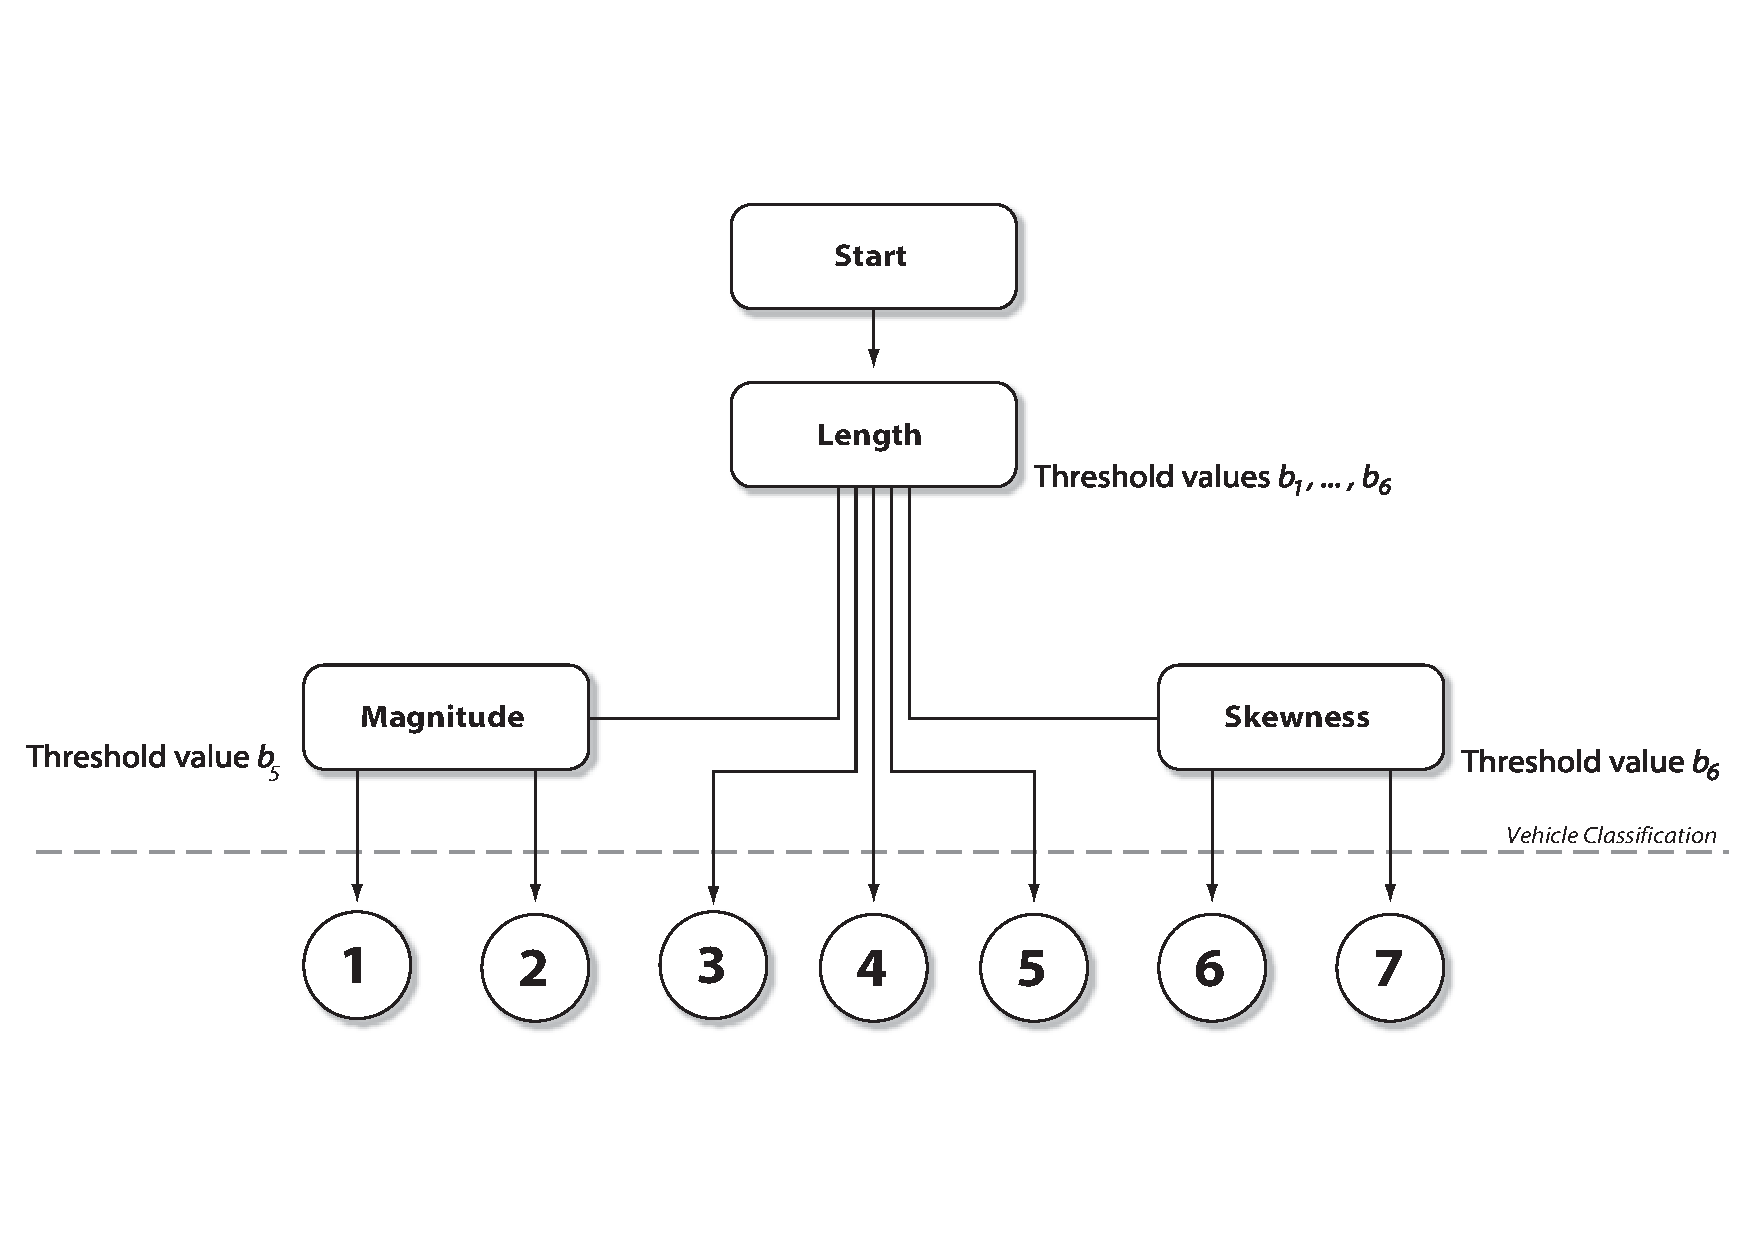
\includegraphics[width=1\linewidth]{images/decision}
 % decision.eps: 1179666x1179666 pixel, 300dpi, 9987.84x9987.84 cm, bb=
 \caption[Decision tree for classification]{Decision tree for classification into seven types of vehicles~\cite{sun2000}.}
 \label{fig:decision}
 \end{minipage}
\end{figure}

\subsection{Hill patterns}\index{hill pattern}
Another way of finding a pattern like the one described in the previous section is to use hill patterns\index{hill pattern}. These are found exactly in the same way as the pattern above, but using the time derivative of the signature. This method has the benefit that we do not need to place the sensor in the middle of the lane but rather at the side of the road. Noise will be an issue with this method, and therefore the signal will need filtering.

The hill pattern is defined~\cite{path2007} as
\begin{align}
 d(n) = \frac{x(nT_s)-x([n-1]T_s)}{T_s},\quad n \in \mathbb{Z}\\
 \overline{d(n)} = \left\{\begin{array}{cl}
+1 & d(n) \geq d_+\\
- 1 & d(n) < d_-\\
0 & \text{otherwise},
\end{array}\right.
\end{align}
where $d_+$ and $d_-$ are the thresholds, positive and negative respectively. Normally they are chosen so that $d_+ = -d_-$.

\subsection{Transforms}
Algorithms based on on discrete Fourier transform\index{discrete Fourier transform}, DFT, and Karhunen-Lo\`{e}ve transform\index{Karhunen-Lo\`{e}ve transform|textbf}, KLT, are proposed in~\cite{sun2000}. In \mbox{Appendix~\ref{chap:plots}} we can find the Fast Fourier Transform, FFT, of the vehicle signatures in each axis. The sensor was placed at the side of the road. We can see that the signatures contain a very different frequency content, and therefore classification could be done using FFT.

% % The Kahunen-Lo\`{e}ve transform is also called the Hotelling transform\index{Hotelling transform|see{Karhunen-Lo\`{e}ve transform}}.
% KLT\cite{papoulis1991}
% \begin{align}
%  \hat{\vec{x}}(t) &= \sum_{n=1}^\infty \vec{c}_n\varphi_n(t) \quad 0<t<T,\\
% \vec{c}_n &= \int_0^T \vec{x}(t)\varphi_n^*(t)\,dt.
% \end{align}
%
%
% The autocorrelation matrix\cite{sayood} for a random process $X$ is defined by
% \begin{equation}
%  [\vec{R}]_{i,j} = E[X_nX_{n+|i-j|}].
% \end{equation}
%
% \begin{align}
%  \vec{Y}^T=\vec{X}^T\vec{W}.
% \end{align}

\subsection{Bins} %yeye
If we do the normalisation and re-sampling as in earlier methods, we can divide the signature into bins. Two examples can be seen in Figures~\ref{fig:bar1} and~\ref{fig:bar2}. We take the mean of the magnitudes in a number of time slots and so we have produced a vector that can be compared with a database. The number of time slots are the same for all vehicles, but the length of each time slot might be different. The length of a signature is an important parameter, and therefore it is necessary to measure that parameter in some way. One way could be to always ``record'' the same signature length, or pad with zeros after the vehicle has passed. Of course we could compare the signature itself with the database entry, but this would require the whole signature to be sent over the WSN, which would perhaps not be effective.

\begin{subfigures}
\begin{figure}
 \centering
 \begin{minipage}{0.45\linewidth}
 \centering
  % generated by laprint.m
% %
% \begin{psfrags}%
% \psfragscanon%
%
% text strings:
\psfrag{s02}[b][b]{\fontsize{8}{12}\fontseries{m}\mathversion{normal}\fontshape{n}\selectfont \setlength{\tabcolsep}{0pt}\begin{tabular}{c}Magnetic Field Strength [nT]\end{tabular}}%
\psfrag{s03}[t][t]{\fontsize{8}{12}\fontseries{m}\mathversion{normal}\fontshape{n}\selectfont \setlength{\tabcolsep}{0pt}\begin{tabular}{c}[bar]\end{tabular}}%
\psfrag{s04}[b][b]{\fontsize{8}{12}\fontseries{m}\mathversion{normal}\fontshape{n}\selectfont \setlength{\tabcolsep}{0pt}\begin{tabular}{c}Average Bar - $\hat{y}$-axis\end{tabular}}%
%
% axes font properties:
\fontsize{6}{12}\fontseries{m}\mathversion{normal}%
\fontshape{n}\selectfont%
%
% xticklabels:
\psfrag{x01}[t][t]{$2$}%
\psfrag{x02}[t][t]{$4$}%
\psfrag{x03}[t][t]{$6$}%
\psfrag{x04}[t][t]{$8$}%
\psfrag{x05}[t][t]{$10$}%
\psfrag{x06}[t][t]{$12$}%
\psfrag{x07}[t][t]{$14$}%
\psfrag{x08}[t][t]{$16$}%
\psfrag{x09}[t][t]{$18$}%
\psfrag{x10}[t][t]{$20$}%
%
% yticklabels:
\psfrag{v01}[r][r]{$-600$}%
\psfrag{v02}[r][r]{$-400$}%
\psfrag{v03}[r][r]{$-200$}%
\psfrag{v04}[r][r]{$0$}%
\psfrag{v05}[r][r]{$200$}%
\psfrag{v06}[r][r]{$400$}%
\psfrag{v07}[r][r]{$600$}%
\psfrag{v08}[r][r]{$800$}%
%
% Figure:
% \resizebox{6cm}{!}{\includegraphics{avb-y.eps}}%
% \end{psfrags}%
%
% End avb-y.tex

  \includegraphics[width=1\linewidth]{images/avb-y}
 % sensoraxis.eps: 1179666x1179666 pixel, 300dpi, 9987.84x9987.84 cm, bb=
 \caption[Average bar - $y$-axis]{Average bar - $y$-axis.}
 \label{fig:bar1}
 \end{minipage}\hfill
 \begin{minipage}{0.45\linewidth}
 \centering
 % generated by laprint.m
% %
% \begin{psfrags}%
% \psfragscanon%
%
% text strings:
\psfrag{s02}[b][b]{\fontsize{8}{12}\fontseries{m}\mathversion{normal}\fontshape{n}\selectfont \setlength{\tabcolsep}{0pt}\begin{tabular}{c}Magnetic Field Strength [nT]\end{tabular}}%
\psfrag{s03}[t][t]{\fontsize{8}{12}\fontseries{m}\mathversion{normal}\fontshape{n}\selectfont \setlength{\tabcolsep}{0pt}\begin{tabular}{c}[bar]\end{tabular}}%
\psfrag{s04}[b][b]{\fontsize{8}{12}\fontseries{m}\mathversion{normal}\fontshape{n}\selectfont \setlength{\tabcolsep}{0pt}\begin{tabular}{c}Average Bar - $\hat{z}$-axis\end{tabular}}%
%
% axes font properties:
\fontsize{6}{12}\fontseries{m}\mathversion{normal}%
\fontshape{n}\selectfont%
%
% xticklabels:
\psfrag{x01}[t][t]{$2$}%
\psfrag{x02}[t][t]{$4$}%
\psfrag{x03}[t][t]{$6$}%
\psfrag{x04}[t][t]{$8$}%
\psfrag{x05}[t][t]{$10$}%
\psfrag{x06}[t][t]{$12$}%
\psfrag{x07}[t][t]{$14$}%
\psfrag{x08}[t][t]{$16$}%
\psfrag{x09}[t][t]{$18$}%
\psfrag{x10}[t][t]{$20$}%
%
% yticklabels:
\psfrag{v01}[r][r]{$0$}%
\psfrag{v02}[r][r]{$500$}%
\psfrag{v03}[r][r]{$1000$}%
\psfrag{v04}[r][r]{$1500$}%
\psfrag{v05}[r][r]{$2000$}%
\psfrag{v06}[r][r]{$2500$}%
\psfrag{v07}[r][r]{$3000$}%
\psfrag{v08}[r][r]{$3500$}%
\psfrag{v09}[r][r]{$4000$}%
%
% % Figure:
% \resizebox{6cm}{!}{\includegraphics{avb-z.eps}}%
% \end{psfrags}%
%
% End avb-z.tex

  \includegraphics[width=1\linewidth]{images/avb-z}
 % sensoraxis.eps: 1179666x1179666 pixel, 300dpi, 9987.84x9987.84 cm, bb=
 \caption[Average bar - $z$-axis]{Average bar - $z$-axis.}
 \label{fig:bar2}
 \end{minipage}
\end{figure}
\end{subfigures}

\subsection{Least-squares estimation}\index{least-squares estimation}\label{subsec:leastsq}
Using least squares analysis we seek to minimise \eqref{eq:leastsq} in order to find the parameters of the magnetic model. This method although very good requires extreme computational power.

\begin{equation}
	S = \sum_i^n \left(y_i - f(\vec{t}_i,\vec{a})\right)^2,\label{eq:leastsq}
\end{equation}
where $y_i$ is the measured data, $f(\vec{t}_i,\vec{a})$ is the output from our model described in Chapter~\ref{chap:model} and $\vec{a}$ is a vector containing the parameters we want to estimate. $\vec{t}_i$ is the time samples, $n$ is the number of samples we have.

The parameters estimated are
\begin{align}
	\vec{\mu}_i &= \left[\,\mu_{x,i}\quad{}\mu_{y,i}\quad{}\mu_{z,i}\,\right]\\
	\vec{r}_i &= \left[\,x_i\quad{}y_i\quad{}z_i\,\right],
\end{align}
and also the speed $v$. It is assumed that the magnetic moments will lie on a straight line, eliminating two degrees of freedom. The vehicle is assumed to be travelling a path perpendicular to the sensor. Three magnetic moments each with four degrees of freedom will have a total of twelve degrees of freedom. Placing one of the magnetic moments in the origin of the vehicle coordinate system will eliminate another degree of freedom. Since the vehicle coordinate system will move, we can add the speed $v$ as another parameter. In all, twelve parameters are estimated from measurements.

\section{Queue Detection}\index{queue detection}
A queue is a number of vehicles that travel slowly close together. This tells us that we can define a function $q(v,d) \geq 0$ where $v$ is the average velocity, and $d$ is the mean distance between vehicles. We can then set a threshold for a function $q(v,d) \in \{0,1\}$ below which we have a queue. A value of 0 means that there are no vehicles on the road, a value of 1 means that the road is completely filled with still-standing vehicles. The mean speed and distance between vehicles can be found in different ways. We can also just see how often the sensor is ``occupied''. A high occupancy means a large number of vehicles, or few slow moving vehicle. We also note that if we are interested in minimising the number of ``catching-up accidents'', just one vehicle is enough to make a very dangerous situation, and therefore it is enough to detect one slow-moving or parked vehicle.

In a queue detection system the nodes need to be complemented by a warning unit. A number of these are presented in \mbox{Appendix~\ref{app:illustrations}} including a flashing unit from \mbox{Amparo SeeMe\mtm}.

No performance analysis will be done for queue detection since velocity estimation forms the basis for queue detection. However, if queue detection will be used the threshold for the  $q(v,d)$ function needs to be trimmed in so that we are not sending a warning too often, or too seldom.
